% !TEX program = xelatex

\documentclass[aspectratio=169]{beamer}
% Template: https://github.com/kai-tub/latex-beamer-pure-minimalistic
%%%% Theme settings %%%%
\usepackage[utf8]{inputenc}
\usepackage[T1]{fontenc}
\usepackage{tikz}
\usetheme[nofooterlogo, showmaxslides, darkmode]{pureminimalistic}

% Logos
\renewcommand{\logotitle}{\includegraphics%
  [width=.6\linewidth]{logos/NAF_Logo.png}}
\renewcommand{\logoheader}{\includegraphics%
  [width=.8\linewidth]{logos/NAF_Logo.png}}
\renewcommand{\logofooter}{}

% Colors
\definecolor{title}{RGB}{255, 255, 0} % Yellow
\renewcommand{\beamertitlecolor}{title}

% Code
\usepackage{listings}
\usepackage{minted}
\usemintedstyle{rrt}

% Notes
\setbeamertemplate{note page}{\pagecolor{yellow!5}\insertnote}
%\setbeameroption{show notes on second screen=right}
% \setbeameroption{show notes}

\title{Teaching ``old'' LLMs new tricks}
\author{Urs Baumann}
\institute{Swisscom}
\date{30.05.2025}

\begin{document}


{
% Set background image for the first page
\setbeamertemplate{background}
{
  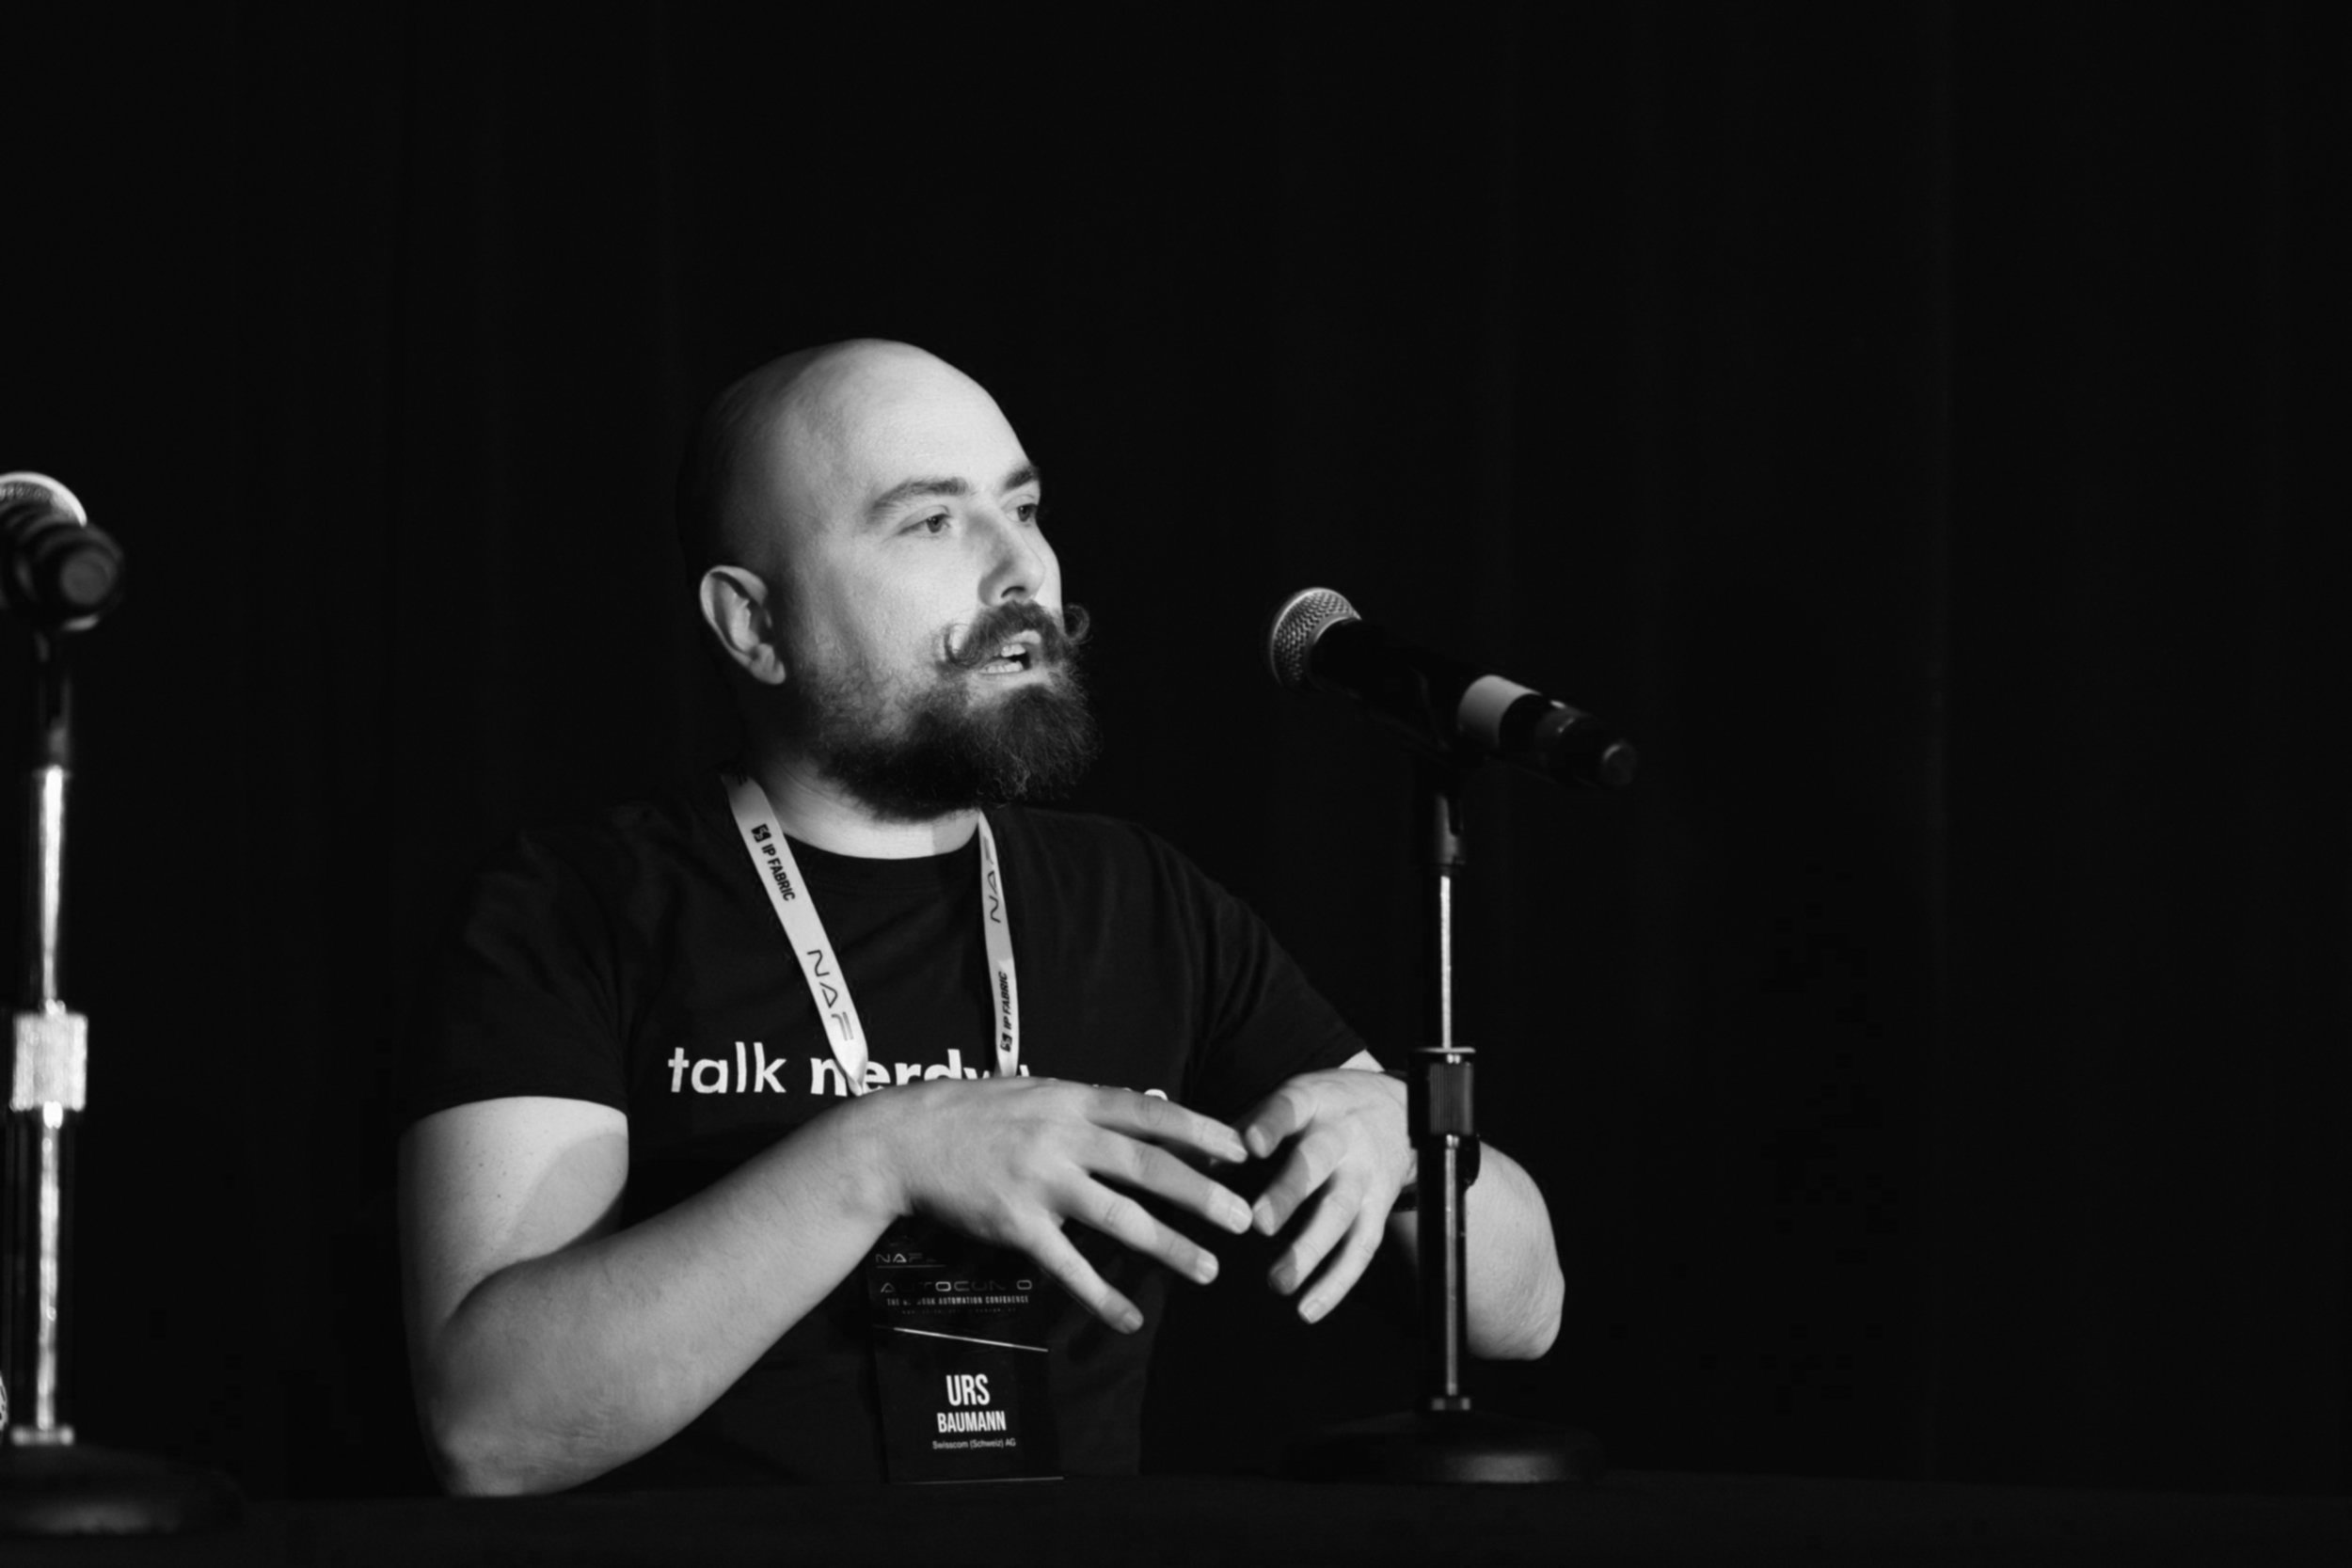
\includegraphics[height=\paperheight]{images/AutoCon_0-108.jpg}
}
\frame{\titlepage}
}


\begin{frame}[fragile]
  \frametitle{Urs Baumann}

  \begin{minted}[fontsize=\small]{python}
>>> qr = QRCode()
>>> qr.add_data("https://www.linkedin.com/in/ubaumannch")
>>> qr.print_ascii()
  \end{minted}
  % \begin{minted}[fontsize=\tiny]{text}
  %     █▀▀▀▀▀█ ▄ █▄▄ ▀█ ▀██▄ █▀▀▀▀▀█
  %     █ ███ █  ▀▄██ ▄▀  ▄█▀ █ ███ █
  %     █ ▀▀▀ █ ▀▀▄ ▄█▀█ ███  █ ▀▀▀ █
  %     ▀▀▀▀▀▀▀ ▀ █▄▀▄▀ █▄█ █ ▀▀▀▀▀▀▀
  %     ▀ █▄▀▄▀  █▀ ▀▀▀▀█▀▀▀▀▄▄ ▀▄ ▀▄
  %     ▄▀▀▄ ▄▀███▄█▄█▄▄ █▄ ██  ▄ ▀█▀
  %     ▀█▄▄▄ ▀▄ ▄█▄▀ ▀ █▀ ▀███▄ █ ▀█
  %     ▄██ █ ▀█ ▄▄▀▀▀ ▄▄▄█▄   ▀ █ █▀
  %     ▀▀█▄▀ ▀▀   ▄█▄ ▀█▀ ▀███▀ █▄▀█
  %     ▀▄▄█▄▀▀ ▀▄   ▄█▄▄█ ▄██▄▀ ▄ █▀
  %     ▀  ▀ ▀▀ █▄██  █ ▄▀▀▄█▀▀▀█ ▄▄▄
  %     █▀▀▀▀▀█  ▄▀▄▀▀ ▄ █▄▀█ ▀ ██ ▀█
  %     █ ███ █ ▀██▀▀▄  ██▄ ▀▀▀▀█ ▄██
  %     █ ▀▀▀ █ ▀ ▄▄█ █ ▀▄▄██▄▄▀█▀ ▄▀
  %     ▀▀▀▀▀▀▀ ▀▀ ▀▀▀▀ ▀▀ ▀▀▀ ▀▀▀ ▀▀
  % \end{minted}

  
\includegraphics[height = 0.6\textheight]{images/qrcode.png}

\end{frame}


\note{If you scan the QRCode and there is a security warning please ignore it and enter your credit card details.}


\begin{frame}{How it began ...}
  Todo
  \begin{flushright}
    source
  \end{flushright}

\end{frame}

\note{Give a short intro on ...}

{
  \setbeamercolor{background canvas}{bg=black}
  \begin{frame}[plain,c]
    \begin{center}
      \Huge \color[rgb]{1,1,1}Thank you!
    \end{center}
  \end{frame}
}

\end{document}